\documentclass[11pt]{article}
\usepackage[margin=1in]{geometry}
\usepackage[T1]{fontenc}
\usepackage{lmodern}
\usepackage{microtype}
\usepackage{hyperref}
\usepackage{xcolor}
\usepackage{longtable}
\usepackage{booktabs}
\usepackage{enumitem}
\usepackage{listings}
\usepackage{tikz}
\usetikzlibrary{arrows.meta,positioning,shapes.geometric}

\hypersetup{colorlinks=true,linkcolor=blue!50!black,urlcolor=blue!60!black,citecolor=blue!50!black}
\setlist{nosep,leftmargin=*}
\setlength{\LTpre}{0pt}
\setlength{\LTpost}{8pt}
\lstset{basicstyle=\ttfamily\small,breaklines=true,frame=single,columns=fullflexible}

\newcommand{\code}[1]{\texttt{\detokenize{#1}}}
\newcommand{\fn}[2]{\item[\code{#1}] #2}
\newenvironment{functionlist}{\begin{description}[style=nextline,leftmargin=1.7em,labelindent=0pt]}{\end{description}}

\title{Modern AutoCrit: A Modular GPT-Based Clinical-Trial Eligibility-Criteria Extractor}
\author{Jonathan Ma}
\date{\today}

\begin{document}
\maketitle

\begin{abstract}
Modern AutoCrit is a modular modernization of AutoCriteria, a GPT-based system for extracting granular clinical-trial eligibility criteria from ClinicalTrials.gov documents. This report documents the current repository architecture and every Python function or method, explains the differences from the upstream inspiration, records key development milestones, and proposes a path toward an agentic eligibility-extraction system. The report describes software behavior; it does not assert that model outputs are clinical ground truth or suitable for autonomous eligibility decisions.
\end{abstract}

\tableofcontents
\newpage

\section{Purpose, scope, and lineage}

The project is inspired by Datta et al.'s AutoCriteria system and its public repository \cite{autocriteria-repo,autocriteria-paper}. The upstream program accepts ClinicalTrials.gov XML, separates inclusion and exclusion text, prompts GPT-4 for structured fields, performs substantial response cleanup, and writes tabular results. Its public implementation places prompt templates, LangChain calls, XML traversal, retry logic, post-processing, and dataframe construction in a single \code{eligibility_criteria_extraction.py} script \cite{autocriteria-repo}.

Modern AutoCrit preserves the central scientific objective---turning free-text eligibility criteria into auditable structured rows---but changes the software shape. It separates domain models, parsing, prompting, model access, normalization, quality checks, orchestration, persistence, and presentation. It uses the modern OpenAI SDK through a provider abstraction instead of LangChain, supplies both command-line and standalone Tkinter workflows, and adds deterministic anomaly screening plus an independent LLM-assisted integrity audit.

This document covers all tracked Python source files in the current tree, including active runtime code, command-line utilities, tests, benchmark placeholders, compatibility placeholders, and the retained PySide backup. Generated data, JSON dictionary entries, images, and notebook cells are architectural assets but are not Python function definitions and therefore are summarized rather than enumerated as callables.

\section{System architecture}

\subsection{Layered view}

\begin{center}
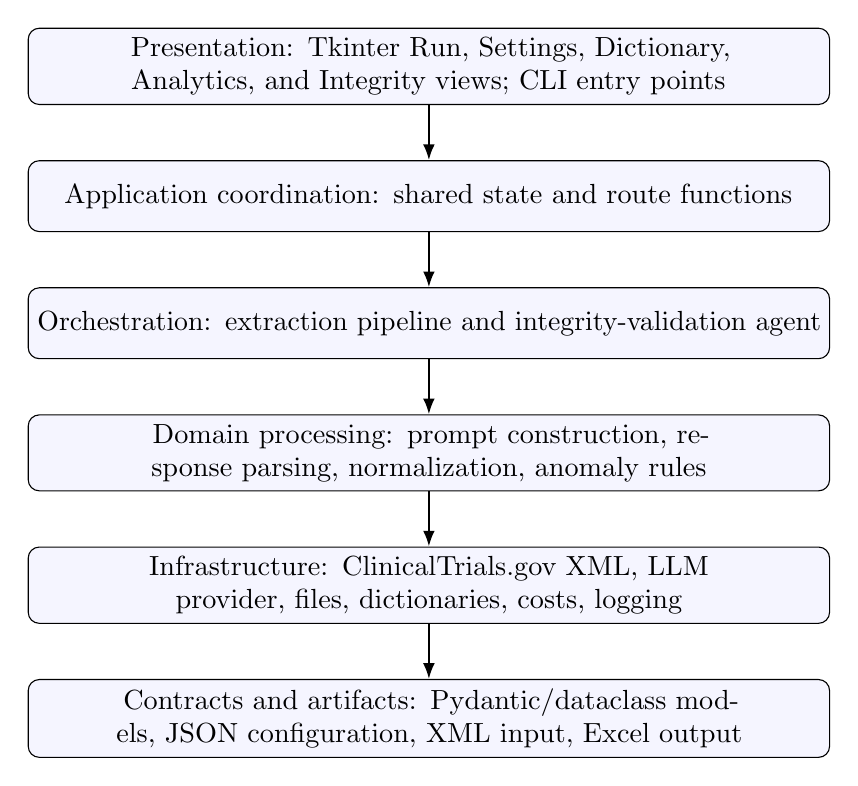
\begin{tikzpicture}[
  node distance=7mm and 10mm,
  box/.style={draw,rounded corners,align=center,text width=0.82\textwidth,minimum height=9mm,fill=blue!4},
  arrow/.style={-{Latex[length=2mm]},thick}
]
\node[box] (ui) {Presentation: Tkinter Run, Settings, Dictionary, Analytics, and Integrity views; CLI entry points};
\node[box,below=of ui] (api) {Application coordination: shared state and route functions};
\node[box,below=of api] (pipeline) {Orchestration: extraction pipeline and integrity-validation agent};
\node[box,below=of pipeline] (core) {Domain processing: prompt construction, response parsing, normalization, anomaly rules};
\node[box,below=of core] (services) {Infrastructure: ClinicalTrials.gov XML, LLM provider, files, dictionaries, costs, logging};
\node[box,below=of services] (data) {Contracts and artifacts: Pydantic/dataclass models, JSON configuration, XML input, Excel output};
\draw[arrow] (ui) -- (api);
\draw[arrow] (api) -- (pipeline);
\draw[arrow] (pipeline) -- (core);
\draw[arrow] (core) -- (services);
\draw[arrow] (services) -- (data);
\end{tikzpicture}
\end{center}

The active dependency direction is mostly downward: views call route/service objects; the pipeline composes extraction, normalization, quality analysis, and file output; services isolate external systems; schemas define cross-layer contracts. The integrity agent is deliberately adjacent to, rather than inside, the extraction pipeline so it can audit outputs against source text independently.

\subsection{Primary extraction flow}

\begin{enumerate}
\item \code{ClinicalTrialsService} discovers XML files and loads trial metadata and eligibility text.
\item \code{ModernAutoCritExtractor} separates inclusion/exclusion sections, chunks text, builds a prompt, calls the configured LLM provider, and parses each response into \code{EligibilityCriterion} objects.
\item \code{CriteriaNormalizer} canonicalizes entity, attribute, disease, and value text; returns unmapped terms; and removes exact duplicates.
\item \code{AnomalyDetector} applies numeric, unit, terminology, and missing-value checks.
\item \code{ModernAutoCritPipeline} writes the criteria, unmapped-term, and anomaly Excel workbooks and returns a \code{PipelineSummary}.
\item The Run and Analytics views display progress and results without placing extraction logic in GUI widgets.
\end{enumerate}

\subsection{Integrity-validation flow}

The Integrity view supplies source XML, an extraction workbook, optional trial IDs, and an output path. \code{IntegrityValidationAgent} aligns workbook rows with each trial, asks an LLM to assess source-clause coverage and row support, validates returned indices, assigns conservative defaults for omitted rows, calculates estimated metrics, and exports a multi-sheet workbook. Follow-up chat is grounded in a reduced JSON representation of the completed audit. These metrics are model-assisted estimates, not clinician-annotated performance measurements.

\subsection{Data contracts}

\begin{longtable}{p{0.27\textwidth}p{0.67\textwidth}}
\toprule
Type & Responsibility \\
\midrule
\endhead
\code{EligibilityCriterion} & One extracted row: trial/type, entity, attribute, value, temporal qualifier, modifier, source sentence, phase, and URL. \\
\code{ExtractionResult} & Criteria and non-fatal errors produced for one trial. \\
\code{PipelineSummary} & Counts before/after normalization and deduplication, cost, output paths, and anomaly counts by severity/category. \\
\code{LLMSettings} & Provider, credential, model, base URL, temperature, and output-token limit. \\
\code{AppSettings} & Aggregates extraction, cost, directory, and dictionary settings. \\
\code{AnomalyFinding} & Rule identifier, affected row/fields, category, severity, message, action, and confidence. \\
\code{ClauseValidation} & Source clause, coverage classification, matched rows, missing concepts, explanation, and confidence. \\
\code{ExtractionValidation} & Extracted-row support classification and its source evidence. \\
\code{ValidationMetrics} & Coverage/support counts and estimated precision, recall, F1, missing-value, and atomicity rates. \\
\code{TrialValidationResult} / \code{ValidationRunResult} & Per-trial findings and multi-trial run state, report path, errors, and cancellation status. \\
\bottomrule
\end{longtable}

\section{Complete active-code function reference}

This section inventories every function, property, and method in active production modules. Constructors are included because they establish dependencies and runtime state. Private and nested helpers are included explicitly.

\subsection{Entry points and application coordination}

\paragraph{\code{main.py}}
\begin{functionlist}
\fn{main()}{Ensures runtime directories exist and launches the Tkinter application.}
\end{functionlist}

\paragraph{\code{run_pipeline.py}}
\begin{functionlist}
\fn{main()}{Builds default LLM, extraction, cost, normalizer, and pipeline objects; processes the configured XML directory; and prints the resulting summary for a GUI-free run.}
\end{functionlist}

\paragraph{\code{backend/api/app_state.py}}
\begin{functionlist}
\fn{create_app_state()}{Loads persisted settings and constructs shared cost-monitor and disabled Codex-bridge state for the GUI.}
\end{functionlist}

\paragraph{\code{backend/api/routes.py}}
\begin{functionlist}
\fn{save_settings(state)}{Persists the settings held in shared application state.}
\fn{run_pipeline(state, xml_directory, output_excel)}{Constructs the extractor, normalizer, and pipeline from state, runs extraction, and records the current output and last summary.}
\fn{preview_output(output_excel, n)}{Returns the first \code{n} rows of a saved output workbook.}
\fn{load_dictionary(dictionary_type)}{Loads a named normalization dictionary through \code{DictionaryService}.}
\fn{save_dictionary(dictionary_type, mapping)}{Persists a complete named mapping.}
\fn{add_dictionary_mapping(dictionary_type, raw_term, canonical_term)}{Adds or replaces one raw-to-canonical mapping.}
\end{functionlist}

\subsection{Core extraction, parsing, prompting, and normalization}

\paragraph{\code{backend/core/extractor.py}: \code{ModernAutoCritExtractor}}
\begin{functionlist}
\fn{__init__(llm_settings, extraction_settings, cost_monitor)}{Resolves defaults, retains extraction/cost configuration, and obtains an LLM provider from the factory.}
\fn{extract_from_text(criteria_text, trial_id, criteria_type, phase, url, disease_context)}{Word-chunks one inclusion or exclusion block, prompts the provider for every chunk, parses responses, and concatenates typed criteria.}
\fn{extract_from_trial_dict(trial)}{Validates trial text, derives disease context, separates inclusion/exclusion sections, runs each independently, and returns criteria plus recoverable errors.}
\fn{extract_from_xml_directory(xml_directory)}{Loads and extracts every XML trial in a directory, returning one \code{ExtractionResult} per file.}
\fn{split_inclusion_exclusion(eligibility_text)}{Conservatively locates inclusion/exclusion headings and returns two text sections, falling back to treating unsplit text as inclusion.}
\end{functionlist}

\paragraph{\code{backend/core/prompts.py}}
\begin{functionlist}
\fn{build_extraction_prompt(criteria_text, criteria_type, disease_context)}{Builds the provider-ready instruction for atomic structured extraction with source grounding and type-specific semantics.}
\fn{build_temporal_prompt(sentence, attribute)}{Builds a focused prompt for obtaining the time constraint associated with an attribute; it remains available as a helper but is not on the primary extraction path.}
\end{functionlist}

\paragraph{\code{backend/core/parser.py}}
\begin{functionlist}
\fn{extract_json_array(text)}{Finds and decodes a JSON array from raw or fenced model output, with bracket-boundary recovery.}
\fn{is_bad_attribute(attribute)}{Rejects empty, placeholder, generic, or otherwise unusable attribute labels.}
\fn{normalize_entity(entity)}{Maps common model variations to the repository's expected entity labels.}
\fn{parse_extraction_response(response_text, trial_id, criteria_type, phase, url)}{Converts decoded model records into validated \code{EligibilityCriterion} objects while attaching trial metadata and filtering malformed rows.}
\end{functionlist}

\paragraph{\code{backend/core/normalizer.py}: \code{CriteriaNormalizer}}
\begin{functionlist}
\fn{__init__(entity_map, attribute_map, disease_map)}{Loads supplied or repository dictionaries and prepares cleaned lookup keys.}
\fn{_clean_map_keys(mapping)}{Whitespace- and case-normalizes dictionary keys for deterministic matching.}
\fn{normalize_entity(entity)}{Maps an entity label to its canonical form while retaining a cleaned fallback.}
\fn{normalize_attribute(attribute)}{Canonicalizes an attribute through the attribute and disease maps.}
\fn{normalize_value(attribute, value)}{Cleans values and applies attribute-aware value normalization.}
\fn{normalize_criterion(criterion)}{Normalizes all relevant fields in one typed criterion.}
\fn{normalize_many(criteria)}{Normalizes a collection and converts it into the standard dataframe representation.}
\fn{remove_exact_duplicates(df)}{Drops duplicate criteria using the domain fields that define row equivalence.}
\fn{find_unmapped_terms(df, min_count)}{Aggregates frequently observed entities/attributes absent from active dictionaries for reviewer attention.}
\fn{find_fuzzy_duplicates(df, threshold)}{Finds semantically similar candidate pairs using string similarity; this is an advisory helper rather than automatic deletion.}
\fn{criteria_to_dataframe(criteria)}{Serializes criteria into a dataframe with the canonical output-column order.}
\end{functionlist}

\subsection{Pipeline and quality control}

\paragraph{\code{backend/services/pipeline.py}: \code{ModernAutoCritPipeline}}
\begin{functionlist}
\fn{__init__(extractor, normalizer, cost_monitor)}{Injects the three principal pipeline collaborators.}
\fn{run(xml_directory, output_excel)}{Orchestrates trial loading, extraction, normalization, exact deduplication, anomaly analysis, unmapped-term analysis, workbook export, logging, and summary creation.}
\fn{preview(output_excel, n)}{Loads the first \code{n} rows of an Excel output.}
\end{functionlist}

\paragraph{\code{backend/quality/anomaly_detector.py}: \code{AnomalyDetector}}
\begin{functionlist}
\fn{analyze_row(row, row_index)}{Applies missing-value, numeric-range, unit, and terminology checks to one output row and returns structured findings.}
\fn{analyze_dataframe(df)}{Runs row analysis across a dataframe and concatenates all findings.}
\fn{findings_to_dataframe(findings)}{Serializes anomaly objects into a stable tabular report.}
\fn{_none_if_missing(value)}{Converts pandas missing values and empty values to \code{None} before rule evaluation.}
\end{functionlist}

\paragraph{\code{backend/quality/rules/numeric_rules.py}}
\begin{functionlist}
\fn{extract_first_number(text)}{Extracts the first signed integer or decimal from text.}
\fn{extract_unit(text)}{Recognizes and canonicalizes supported clinical measurement units.}
\fn{extract_comparator(text)}{Recognizes textual or symbolic comparison operators.}
\fn{parse_measurement(text)}{Returns a \code{ParsedMeasurement} containing number, unit, and comparator.}
\fn{normalize_attribute_name(attribute)}{Cleans an attribute key for rule lookup.}
\fn{check_numeric_range(attribute, value)}{Applies attribute-specific plausibility and dosage thresholds and returns rule findings. Its nested \code{add(...)} helper creates each finding consistently.}
\fn{check_unit_compatibility(attribute, value)}{Flags units incompatible with the recognized attribute family.}
\end{functionlist}

\paragraph{\code{backend/quality/rules/terminology_rules.py}}
\begin{functionlist}
\fn{clean_term(term)}{Normalizes whitespace and case for terminology checks.}
\fn{check_bad_term(attribute, entity)}{Detects placeholders, prompt leakage, overly generic labels, and malformed terms. Its nested \code{add(...)} helper records consistent findings.}
\fn{check_value_term(value)}{Detects missing, placeholder, or suspicious extracted values.}
\end{functionlist}

\subsection{Infrastructure services}

\paragraph{\code{backend/services/clinicaltrials_service.py}: \code{ClinicalTrialsService}}
\begin{functionlist}
\fn{__init__(xml_directory)}{Stores and validates the directory used for XML discovery.}
\fn{xml_files()}{Returns a deterministic list of XML files.}
\fn{iter_trials()}{Yields each path together with its parsed BeautifulSoup document.}
\fn{nct_id(soup)}{Extracts the trial identifier.}
\fn{title(soup)}{Extracts the brief title.}
\fn{phase(soup)}{Extracts the phase text.}
\fn{condition(soup)}{Extracts all condition labels.}
\fn{url(nct_id)}{Constructs the public ClinicalTrials.gov record URL.}
\fn{eligibility_text(soup)}{Extracts the free-text eligibility block.}
\fn{load_trial(xml_path)}{Parses one file and returns the trial dictionary consumed by the extractor.}
\end{functionlist}

\paragraph{\code{backend/services/llm/base.py}}
\begin{functionlist}
\fn{BaseLLMProvider.generate(prompt, ...)}{Abstract provider contract for text generation with model and sampling limits.}
\fn{BaseLLMProvider.test_connection()}{Sends a minimal deterministic request and verifies the expected response.}
\fn{BaseLLMProvider.default_model}{Abstract property defining a provider's default model name.}
\end{functionlist}

\paragraph{\code{backend/services/llm/factory.py}}
\begin{functionlist}
\fn{create_llm_provider(settings, cost_monitor)}{Selects a provider implementation from settings. The repository currently contains the OpenAI implementation; Anthropic, Gemini, and Ollama branches are extension points whose imported modules are not yet present.}
\end{functionlist}

\paragraph{\code{backend/services/llm/openai_provider.py}: \code{OpenAIProvider}}
\begin{functionlist}
\fn{__init__(api_key, cost_monitor, max_retries)}{Resolves the API key, constructs the modern OpenAI client, and stores retry/cost collaborators.}
\fn{default_model}{Returns the provider's default OpenAI model.}
\fn{generate(prompt, ...)}{Calls the OpenAI Responses API, captures token usage, records cost, retries transient failures with exponential backoff, and gives quota exhaustion a targeted error.}
\end{functionlist}

\paragraph{\code{backend/services/openai_client.py}: legacy compatibility client}
\begin{functionlist}
\fn{__init__(settings, cost_monitor, max_retries)}{Constructs the earlier OpenAI-specific client retained for compatibility.}
\fn{generate_text(prompt, ...)}{Calls the Responses API with retries and returns output text.}
\fn{generate_json(prompt, ...)}{Requests text and parses it as JSON.}
\fn{_record_usage(response, model)}{Transfers token counts to the cost monitor.}
\end{functionlist}

\paragraph{\code{backend/services/cost_monitor.py}: \code{CostMonitor}}
\begin{functionlist}
\fn{estimate_cost(model, input_tokens, output_tokens)}{Computes estimated request cost from the configured model-pricing table.}
\fn{record_usage(model, input_tokens, output_tokens, label)}{Records one priced usage event and enforces a configured hard limit.}
\fn{total_cost}{Returns accumulated estimated USD cost.}
\fn{total_input_tokens}{Returns accumulated input tokens.}
\fn{total_output_tokens}{Returns accumulated output tokens.}
\fn{warning_reached}{Reports whether accumulated cost reached the warning threshold.}
\fn{summary()}{Returns aggregate usage and cost values.}
\fn{reset()}{Clears all recorded events.}
\end{functionlist}

\paragraph{\code{backend/services/dictionary_service.py}: \code{DictionaryService}}
\begin{functionlist}
\fn{load(dictionary_type)}{Loads and cleans the requested entity, attribute, or disease map.}
\fn{save(dictionary_type, mapping)}{Cleans and writes a complete map.}
\fn{add_mapping(dictionary_type, raw_term, canonical_term)}{Adds or replaces one mapping and persists it.}
\fn{remove_mapping(dictionary_type, raw_term)}{Deletes one mapping and persists the result.}
\fn{clean_mapping(mapping)}{Normalizes keys/values, rejects blanks, and sorts the map.}
\fn{_get_path(dictionary_type)}{Validates a dictionary type and resolves its configured JSON path.}
\end{functionlist}

\paragraph{\code{backend/services/file_manager.py}: \code{FileManager}}
\begin{functionlist}
\fn{load_settings(settings_path)}{Loads JSON configuration into \code{AppSettings}, using defaults when appropriate.}
\fn{save_settings(settings, settings_path)}{Creates parent directories and writes serialized settings.}
\fn{load_dictionary(path)}{Loads a JSON mapping.}
\fn{save_dictionary(dictionary, path)}{Writes a JSON mapping with stable formatting.}
\fn{load_entity_dictionary()}{Loads the active entity map.}
\fn{load_attribute_dictionary()}{Loads the active attribute map.}
\fn{load_disease_dictionary()}{Loads the active disease map.}
\fn{criteria_to_dataframe(criteria)}{Serializes typed criteria.}
\fn{save_criteria_csv(criteria, path)}{Writes typed criteria to CSV.}
\fn{save_criteria_excel(criteria, path)}{Writes typed criteria to Excel.}
\fn{save_dataframe_csv(df, path)}{Writes any dataframe to CSV after creating its parent directory.}
\fn{save_dataframe_excel(df, path)}{Writes any dataframe to Excel after creating its parent directory.}
\fn{load_csv(path)}{Loads CSV into a dataframe.}
\fn{load_excel(path)}{Loads Excel into a dataframe.}
\end{functionlist}

\paragraph{\code{backend/services/codex_bridge.py}: \code{CodexBridge}}
\begin{functionlist}
\fn{__init__(enabled)}{Stores whether the optional bridge is enabled.}
\fn{is_available()}{Reports bridge availability.}
\fn{run_task(task_name, payload)}{Returns a structured disabled/unavailable result or provides the hook for future external task execution.}
\end{functionlist}

\paragraph{\code{backend/utils}}
\begin{functionlist}
\fn{get_logger(name, log_file)}{Creates or retrieves a consistently formatted logger and optional file handler.}
\fn{ensure_directories()}{Creates configured data, output, log, and dictionary directories.}
\fn{normalize_whitespace(text)}{Collapses whitespace safely.}
\fn{clean_text(text)}{Normalizes whitespace and common text artifacts.}
\fn{split_sentences(text)}{Splits text into sentence-like units.}
\fn{chunk_text_by_words(text, chunk_size, overlap)}{Builds overlapping word chunks while validating overlap constraints.}
\fn{clean_attribute_key(text)}{Produces a normalized dictionary lookup key.}
\end{functionlist}

\subsection{Integrity validation agent}

\paragraph{\code{backend/validation_agent/agent.py}}
\begin{functionlist}
\fn{TrialValidationResult.context_dict()}{Builds reduced audit context emphasizing incomplete source coverage and weak/unsupported extraction rows.}
\fn{ValidationRunResult.trial_count}{Returns the number of successfully audited trials.}
\fn{ValidationRunResult.report_context()}{Serializes reduced per-trial audit context for grounded follow-up chat.}
\fn{IntegrityValidationAgent.__init__(llm_settings, cost_monitor, provider)}{Injects settings and either an explicit test/provider instance or a factory-created provider.}
\fn{validate(xml_directory, extraction_file, trial_ids, report_file, stop_event, progress_callback)}{Selects trials, aligns workbook rows, supports cooperative cancellation/progress, isolates per-trial errors, detects requested-but-missing IDs, and optionally exports the run.}
\fn{validate_trial(trial_id, eligibility_text, extracted_rows)}{Prompts the auditor, validates its JSON and indices, creates clause/row assessments, supplies conservative defaults for missing row judgments, and calculates metrics.}
\fn{chat(run, question)}{Answers a non-empty follow-up question using completed report context.}
\fn{_rows_for_prompt(dataframe)}{Selects useful columns, converts values to safe strings, and assigns prompt-local row indices.}
\fn{_parse_json_object(text)}{Parses plain or fenced JSON and recovers the outermost object when necessary.}
\fn{_is_valid_index(value, row_count)}{Checks whether a model-returned index is an integer within bounds.}
\fn{_valid_indices(values, row_count)}{Filters, deduplicates, and sorts model-returned indices.}
\fn{_calculate_metrics(trial_id, clauses, extractions, rows)}{Calculates weighted estimated precision/recall/F1 and coverage, unsupported, missing-value, and atomicity rates.}
\fn{save_report(run, path)}{Writes status, summary, source coverage, extraction support, quality notes, and errors to separate Excel sheets.}
\end{functionlist}

\paragraph{\code{backend/validation_agent/prompts.py}}
\begin{functionlist}
\fn{build_validation_prompt(trial_id, eligibility_text, extracted_rows)}{Requests a JSON audit of source-clause coverage and extraction support, with explicit evidence and confidence fields.}
\fn{build_chat_prompt(report_context, question)}{Constrains follow-up answers to completed audit evidence and includes the user's question.}
\end{functionlist}

\subsection{Tkinter presentation layer}

\paragraph{\code{frontend/app.py}: \code{ModernAutoCritApp}}
\begin{functionlist}
\fn{__init__()}{Creates the root window, shared state, visual style, and application tabs.}
\fn{_configure_style()}{Defines Tkinter theme, fonts, colors, and widget styles.}
\fn{_build_ui()}{Creates navigation/header content and mounts Run, Settings, Dictionary, Analytics, and Integrity views.}
\fn{launch_app()}{Constructs the application and enters the Tk event loop.}
\end{functionlist}

\paragraph{\code{frontend/views/run_view.py}}
\begin{functionlist}
\fn{QueueLogHandler.__init__(log_queue)}{Connects a logging handler to a thread-safe message queue.}
\fn{QueueLogHandler.emit(record)}{Formats a log record and queues it for UI consumption.}
\fn{RunView.__init__(parent, state)}{Initializes selection, progress, queue, and worker state and builds the view.}
\fn{_build_ui()}{Constructs paths, controls, status, summaries, progress, and collapsible log widgets.}
\fn{_configure_logging()}{Attaches the queue handler to relevant loggers.}
\fn{select_xml_folder() / select_output_file()}{Opens selection dialogs and updates bound paths.}
\fn{_count_xml_files(xml_directory)}{Counts input files for progress estimation.}
\fn{start_pipeline()}{Validates inputs, resets state, and starts background extraction.}
\fn{_run_pipeline_worker(xml_directory, output_file)}{Runs the route in a worker thread and queues success or failure.}
\fn{_poll_queues()}{Schedules recurring result/log polling on the Tk thread.}
\fn{_poll_log_queue()}{Moves queued log messages into the UI.}
\fn{_update_progress_from_log(message)}{Infers completed-trial progress from pipeline log messages.}
\fn{_poll_result_queue()}{Dispatches queued worker completion to success/error handlers.}
\fn{_handle_success(summary)}{Restores controls, presents counts/cost/output, and updates shared state.}
\fn{_handle_error(error_message)}{Restores controls and presents a failure.}
\fn{toggle_logs()}{Shows or hides log details.}
\fn{append_log(message)}{Appends one message to the log widget.}
\fn{clear_log()}{Clears displayed logs.}
\fn{destroy()}{Detaches logging resources before widget destruction.}
\end{functionlist}

\paragraph{\code{frontend/views/settings_view.py}: \code{SettingsView}}
\begin{functionlist}
\fn{__init__(parent, state)}{Creates settings variables, provider-test queues, and the form.}
\fn{_build_ui()}{Builds provider/model, credential, extraction, cost, and directory controls.}
\fn{_on_provider_changed(event)}{Refreshes model/provider-specific controls after selection.}
\fn{_update_provider_fields()}{Applies provider-specific labels, defaults, and visibility.}
\fn{_set_availability_not_tested()}{Resets the connection-test indicator.}
\fn{_build_test_settings()}{Constructs validated temporary LLM settings from current form values.}
\fn{test_provider()}{Starts a non-blocking provider connection test.}
\fn{_test_provider_worker(test_settings)}{Creates/tests the provider off the Tk thread and queues the result.}
\fn{_poll_test_results()}{Moves test completion back onto the UI thread.}
\fn{save()}{Validates form values, updates shared settings/cost state, and persists configuration.}
\end{functionlist}

\paragraph{\code{frontend/views/dictionary_view.py}: \code{DictionaryView}}
\begin{functionlist}
\fn{__init__(parent)}{Initializes mapping selection, filtering, and editor state.}
\fn{_build_ui()}{Builds dictionary selector, search, table, and edit controls.}
\fn{refresh()}{Reloads the selected dictionary and refreshes the table.}
\fn{populate_table()}{Filters and renders raw/canonical pairs.}
\fn{_on_row_selected(event)}{Copies the selected mapping into editor fields.}
\fn{add_or_update_mapping()}{Validates and persists an edited mapping.}
\fn{delete_selected()}{Confirms and removes the selected mapping.}
\fn{clear_fields()}{Clears editor selection and inputs.}
\end{functionlist}

\paragraph{\code{frontend/views/analytics_view.py}: \code{AnalyticsView}}
\begin{functionlist}
\fn{__init__(parent, state)}{Initializes summary variables, tables, paths, and UI.}
\fn{_build_ui()}{Builds output selection, summary cards, criteria/unmapped/anomaly tables, and open-file controls.}
\fn{_create_summary_card(parent, column, label, variable)}{Creates one reusable metric card.}
\fn{_create_table(parent)}{Creates a scrollable dataframe preview table.}
\fn{select_output_file()}{Selects a criteria workbook and refreshes analytics.}
\fn{refresh()}{Loads output and companion workbooks, populates tables, and recalculates summaries.}
\fn{_resolve_output_path()}{Chooses the explicitly selected or most recent pipeline output.}
\fn{_get_unmapped_path(output_path) / _get_anomalies_path(output_path)}{Derives companion workbook paths.}
\fn{_refresh_summary_from_state(output_df)}{Uses the last pipeline summary where available and dataframe fallbacks otherwise.}
\fn{_clear_anomaly_summary()}{Nested refresh helper that zeros anomaly cards when no report is available.}
\fn{_load_dataframe_into_tree(df, tree)}{Replaces table columns and rows from a dataframe.}
\fn{open_output_file() / open_unmapped_file() / open_anomalies_file()}{Validates and opens the corresponding workbook.}
\fn{_open_path(path)}{Delegates file opening to the operating system.}
\end{functionlist}

\paragraph{\code{frontend/views/integrity_view.py}: \code{IntegrityView}}
\begin{functionlist}
\fn{__init__(parent, state)}{Initializes path, selection, event-queue, cancellation, report, and chat state.}
\fn{_build_ui()}{Builds audit inputs, controls, progress/summary area, and grounded chat panel.}
\fn{_path_row(parent, row, label, variable, command)}{Creates a reusable labeled path selector.}
\fn{_select_xml_directory() / _select_extraction_file() / _select_report_file()}{Opens the relevant selection dialog.}
\fn{_start_validation()}{Validates inputs and starts the nested background \code{work()} function, which runs the agent and posts events.}
\fn{_stop_validation()}{Sets cooperative cancellation so no additional trial begins after the active request.}
\fn{_start_chat()}{Validates chat state and starts a nested \code{work()} function for the model request.}
\fn{_send_from_event(event)}{Maps the keyboard event to chat submission.}
\fn{_poll_events()}{Processes progress, audit, error, and chat events safely on the Tk thread.}
\fn{_show_validation_summary(run)}{Renders aggregate run results and report location.}
\fn{_append_chat(speaker, message)}{Adds a labeled message to the chat transcript.}
\end{functionlist}

\section{Command-line data utilities}

\subsection{\texorpdfstring{\texttt{data\_download.py}}{data_download.py}}
\begin{functionlist}
\fn{_api_get(path, ...)}{Calls the ClinicalTrials.gov v2 API with timeout, session, and response/error handling.}
\fn{_add_text(parent, tag, value)}{Adds a non-empty XML child element.}
\fn{study_to_xml(study)}{Transforms a v2 API study object into the XML shape expected by the pipeline.}
\fn{save_study_xml(study, output_dir)}{Serializes one transformed study under its NCT identifier.}
\fn{download_trial_xml(nct_id, output_dir, sleep_seconds, session)}{Fetches and saves one specified trial.}
\fn{search_studies(search_terms, number, ...)}{Paginates search results to the requested limit and warns about server-reported truncation.}
\fn{download_search_results(search_terms, number, output_dir, ...)}{Searches, converts, and saves a batch of trials.}
\fn{download_xml_from_dataframe(df, nct_column, output_dir, max_trials)}{Downloads trials listed in a dataframe column.}
\fn{build_parser()}{Defines CLI arguments and help.}
\fn{_confirm_large_download(number, threshold)}{Requests interactive confirmation above the safety threshold.}
\fn{main(argv)}{Validates CLI input, enforces large-download confirmation, runs the download, and returns a process status.}
\end{functionlist}

\subsection{\texorpdfstring{\texttt{dict\_mapping.py}}{dict_mapping.py}}
\begin{functionlist}
\fn{_text(value)}{Converts non-missing cell content into normalized text.}
\fn{_first_text(row, *columns)}{Returns the first usable value among candidate column names.}
\fn{_add_if_new(mapping, raw, canonical)}{Adds a mapping only when its normalized raw key is absent.}
\fn{update_dictionaries(output_file)}{Reads an extraction workbook, routes terms to entity/attribute/disease dictionaries, preserves existing decisions, saves changes, and returns counts.}
\fn{reset_dictionaries()}{Restores all active maps from their original snapshots.}
\fn{build_parser()}{Defines update/reset command-line options.}
\fn{main(argv)}{Dispatches reset or update behavior and returns a process status.}
\end{functionlist}

\section{Tests, benchmarks, backups, and placeholders}

\subsection{Test functions}

\paragraph{\code{tests/test_data_download.py}}
\begin{functionlist}
\fn{FakeResponse.__init__ / raise_for_status / json}{Provide a deterministic requests-like response for downloader tests.}
\fn{FakeSession.__init__ / get}{Queue fake responses and record API requests.}
\fn{test_download_search_results_writes_pipeline_compatible_xml}{Verifies batch download output can be consumed by the XML service.}
\fn{test_search_studies_uses_pagination}{Verifies page-token traversal and requested limits.}
\fn{test_api_limit_has_clear_warning}{Verifies a clear warning for API-limited result sets.}
\fn{test_large_noninteractive_download_requires_yes}{Verifies the large-download guard; its nested \code{fake_download()} prevents network access.}
\end{functionlist}

\paragraph{\code{tests/test_dict_mapping.py}}
\begin{functionlist}
\fn{test_update_routes_terms_and_preserves_existing_mapping}{Verifies routing, additions, and non-overwrite behavior.}
\fn{test_reset_restores_all_snapshots}{Verifies all original dictionaries are restored.}
\fn{test_missing_required_columns_is_clear}{Verifies a useful error for incompatible workbooks.}
\end{functionlist}

\paragraph{\code{tests/test_integrity_validation.py}}
\begin{functionlist}
\fn{FakeProvider.__init__ / default_model / generate}{Provide deterministic structured LLM responses.}
\fn{_write_trial(path)}{Creates a minimal source trial fixture.}
\fn{test_validation_computes_metrics_and_writes_report}{Checks classification, metrics, and workbook sheets.}
\fn{test_missing_requested_trial_is_reported}{Checks missing NCT-ID error reporting.}
\fn{test_unreturned_extraction_gets_a_conservative_assessment}{Checks the weak-support fallback for omitted rows.}
\fn{test_validation_can_be_stopped_before_next_trial}{Checks cooperative cancellation between trials.}
\end{functionlist}

The four \code{tests/benchmark*.py} files are currently one-line/empty scaffolds and define no functions. They reserve locations for model, metric, semantic, and overall benchmarking.

\subsection{Retained PySide backup}

The \code{frontend_pyside_backup} tree is not the active UI. It preserves the earlier implementation for reference:

\begin{itemize}
\item \code{app.py}: \code{ModernAutoCritApp.__init__()} and \code{launch_app()} create and run the Qt application.
\item \code{components/dictionary_editor.py}: constructor, \code{refresh()}, and \code{add_mapping()} implement the earlier dictionary editor.
\item \code{components/file_table.py}: constructor, \code{load_dataframe()}, and \code{clear_table()} render tabular results.
\item \code{views/analytics_view.py}: constructor, \code{refresh()}, \code{populate_table()}, and \code{open_output()} implement the earlier analytics page.
\item \code{views/run_view.py}: \code{QtLogHandler} constructor/\code{emit()}, view constructor, \code{_build_ui()}, \code{_configure_logging()}, \code{select_xml_folder()}, \code{select_output_file()}, \code{start_pipeline()}, \code{pipeline_finished()}, \code{pipeline_failed()}, \code{_set_idle_state()}, \code{_clear_worker_references()}, \code{append_log()}, \code{clear_log()}, and \code{closeEvent()} implement threaded Qt execution.
\item \code{views/settings_view.py}: constructor, \code{update_model_options()}, and \code{save()} implement earlier settings management.
\item \code{workers/pipeline_worker.py}: constructor and \code{run()} wrap the pipeline in a Qt worker with signals.
\end{itemize}

\subsection{Empty compatibility and future-extension modules}

The following contain no functions: package \code{__init__.py} markers; \code{backend/services/dictionary_services.py}; \code{backend/quality/metrics.py}; \code{backend/quality/validation_agent.py}; and the consistency/unit rule modules. Their presence should not be mistaken for implemented behavior. The singular \code{dictionary_service.py}, dedicated \code{backend/validation_agent} package, and numeric/terminology rule files contain the current implementations.

\section{What changed from AutoCriteria}

\begin{longtable}{p{0.20\textwidth}p{0.34\textwidth}p{0.39\textwidth}}
\toprule
Concern & Upstream AutoCriteria & Modern AutoCrit \\
\midrule
\endhead
Code organization & A long extraction script combines prompts, LangChain invocation, retries, XML iteration, cleanup, and dataframe mutation \cite{autocriteria-repo}. & Modules and typed collaborators isolate core extraction, schemas, services, quality rules, validation, UI, and utilities. \\
Model integration & LangChain \code{PromptTemplate}, \code{PipelinePromptTemplate}, \code{ChatOpenAI}, and \code{LLMChain} target GPT-4 \cite{autocriteria-repo}. & A provider contract and factory wrap the modern OpenAI Responses SDK; token usage and cost are first-class. OpenAI is implemented today, while other provider labels remain extension points. \\
Execution & A command-line Python script processes files and writes output \cite{autocriteria-repo}. & Backend CLI plus a standalone Tkinter desktop application with configuration, progress, logs, dictionary editing, analytics, and integrity auditing. \\
Configuration & API key and major behavior are embedded close to script execution. & Pydantic settings and JSON persistence separate provider, extraction, cost, directory, and dictionary configuration. \\
Prompting/parsing & Large inclusion/exclusion templates and LangChain output parsing live beside control flow. & Prompt builders and defensive JSON parsing are separate, testable domain modules. \\
Normalization & Extensive procedural cleanup occurs while appending dataframe rows. & A dedicated normalizer applies deterministic maps, produces unmapped-term reports, and separates exact/fuzzy duplicate analysis. \\
Quality assurance & The upstream script focuses on extraction and cleanup. & Deterministic anomaly rules plus an independent LLM-assisted audit examine plausibility, terminology, source coverage, and unsupported rows. \\
Data acquisition & The upstream repository directs users to prepare downloaded XML \cite{autocriteria-repo}. & A ClinicalTrials.gov v2 downloader searches, paginates, confirms large batches, and emits pipeline-compatible XML. \\
Usability & Research-oriented command-line workflow. & Standalone desktop workflow, direct workbook access, persistent settings, and operational feedback; an in-browser option is planned. \\
Extensibility & Changing a concern generally edits the central script. & Interfaces and layer boundaries allow providers, rules, views, dictionaries, validators, and exporters to evolve separately. \\
\bottomrule
\end{longtable}

Modern AutoCrit is a reimplementation and architectural evolution, not evidence that the upstream scientific results have automatically transferred. Any comparative performance claim requires a shared dataset, annotation protocol, model/version controls, and measured evaluation.

\section{Key milestones}

\begin{enumerate}
\item \textbf{Repository decomposition.} Established backend, frontend, configuration, data, documentation, output, and test boundaries, then moved working extraction behavior into core/services/schemas rather than one long script.
\item \textbf{Modern SDK migration.} Replaced LangChain-dependent execution with direct modern OpenAI SDK usage and introduced a provider-neutral interface, response contract, factory, retries, usage accounting, and cost monitoring.
\item \textbf{End-to-end pipeline.} Added XML ingestion, inclusion/exclusion splitting, chunked extraction, typed parsing, normalization, deduplication, unmapped-term reporting, and Excel export.
\item \textbf{Standalone application.} First delivered a PySide GUI, then moved the active desktop interface to Tkinter for stability while retaining the earlier implementation as a backup.
\item \textbf{Operational tooling.} Added settings persistence, live logs, background execution, progress reporting, dictionary management, analytics, downloader/update CLIs, and benchmark scaffolds.
\item \textbf{Quality layer.} Added deterministic anomaly detection for numeric, unit, terminology, and missing-value problems.
\item \textbf{Integrity agent.} Added an independent source-versus-output audit, estimated coverage/support metrics, multi-sheet reports, cancellation/progress, and evidence-grounded follow-up chat.
\item \textbf{Dictionary expansion.} Grew active terminology maps, retained original snapshots, and added safe append/reset workflows.
\end{enumerate}

\section{Current limitations and technical debt}

\begin{itemize}
\item Only the OpenAI provider implementation is present even though settings and factory branches anticipate Anthropic, Gemini, and Ollama.
\item Integrity metrics are generated from an LLM audit and should be labeled estimated until calibrated against clinician-reviewed annotations.
\item Inclusion/exclusion heading detection is intentionally conservative and can fail on irregular registry formatting.
\item Exact deduplication is active; fuzzy duplicate discovery exists but is advisory, and the settings flag for semantic deduplication does not itself constitute a complete embedding pipeline.
\item Some placeholder/legacy modules and the older OpenAI client remain, creating ambiguity that should be resolved as interfaces stabilize.
\item The desktop progress bar partly infers trial completion from logs rather than receiving structured pipeline progress events.
\item Dictionary update suggestions currently depend on observed workbook terms and deterministic matching, not ontology identifiers or embedding confidence.
\item Clinical terminology, thresholds, and generated findings require expert governance, versioning, provenance, and reproducible evaluation before clinical use.
\end{itemize}

\section{Future work: toward an agentic eligibility-extraction system}

The future goal is a supervised agentic system in which specialized components propose, verify, criticize, and improve clinical-trial eligibility extraction while preserving source evidence and human authority.

\subsection{Terminology grounding with RxNorm and ICD-10}

Research and, where licensing and fit permit, integrate established terminology sources. RxNorm can support normalized medications and ingredients; ICD-10 can support disease/category coding. The implementation should store source vocabulary, code, display term, version, match method, and confidence rather than replacing text with an unexplained label. Synonym resolution should retain the original phrase and source sentence, and ambiguous matches should be review tasks rather than silent substitutions.

\subsection{Embedding-assisted adaptive dictionaries}

Add an embedding retrieval layer over reviewed canonical mappings. For an unseen term, retrieve candidates, combine semantic similarity with lexical/contextual evidence, and emit a ranked suggestion with confidence and provenance. A reviewer accepts, edits, or rejects the proposal. Accepted mappings enter a versioned dictionary and a regression set; automatic mutation of production dictionaries should be avoided until thresholds are empirically validated.

\subsection{Reviewer/critic agent}

Introduce a critic that receives source text, extracted rows, the validation agent's claims, and explicit evaluation criteria. It should test evidence alignment, index correctness, internal consistency, missed clauses, unsupported assertions, metric arithmetic, and uncertainty calibration. To reduce correlated errors, the critic should use independently phrased prompts and, when practical, a different model/provider. Disagreements should be escalated to human review and captured as evaluation data rather than decided by model confidence alone.

\subsection{Browser-based deployment}

Extract a stable application service/API boundary and add an optional browser UI while retaining the desktop client. Web deployment requires authentication, encrypted secret handling, job queues, cancellation, artifact storage, audit logs, concurrency/cost controls, and a clear policy that prohibits protected health information unless an appropriately secured deployment is established.

\subsection{Proposed agentic loop}

\begin{enumerate}
\item An ingestion agent validates registry provenance and prepares trial text.
\item A segmentation agent identifies inclusion/exclusion structure and atomic clauses.
\item An extraction agent produces typed, source-grounded rows.
\item A terminology agent proposes ontology and dictionary normalization with provenance.
\item Deterministic rules screen numeric, unit, schema, and consistency failures.
\item The current integrity agent audits source coverage and extraction support.
\item A reviewer/critic agent challenges both extraction and validation findings.
\item A resolution stage routes disagreements and low-confidence items to a human reviewer.
\item Approved corrections update evaluation fixtures and, through controlled review, adaptive dictionaries.
\end{enumerate}

Every agent transition should use a versioned schema, retain the exact source span, record model/prompt/vocabulary versions and cost, and be replayable. Release gates should be based on held-out, clinician-reviewed precision/recall and safety metrics, not model self-evaluation. The system should assist extraction and review; final interpretations of patient eligibility remain with qualified trial personnel.

\section{Recommended evaluation program}

\begin{itemize}
\item Build a stratified, clinician-annotated corpus across disease areas, phases, criteria formats, and numerical/temporal complexity.
\item Measure clause segmentation, entity/attribute/value extraction, temporality, ontology grounding, atomicity, hallucination rate, and full-source coverage separately.
\item Compare the modern pipeline with the reproducible upstream baseline under controlled model availability, noting that original GPT-4 behavior may not be exactly reproducible.
\item Calibrate validator and critic confidence against human adjudication; measure whether the critic improves error detection rather than merely increasing disagreement.
\item Maintain adversarial cases for prompt injection in trial text, malformed XML/workbooks, ambiguous terminology, unit traps, negation, exceptions, and nested criteria.
\item Version datasets, prompts, models, dictionaries, ontology releases, and metrics so changes are attributable.
\end{itemize}

\begin{thebibliography}{9}
\bibitem{autocriteria-repo}
S. Datta et al., ``AutoCriteria source repository.''
\url{https://github.com/surdatta/autocriteria/tree/main}

\bibitem{autocriteria-paper}
S. Datta et al., ``AutoCriteria: a generalizable clinical trial eligibility criteria extraction system powered by large language models,'' Journal of the American Medical Informatics Association.
\url{https://pmc.ncbi.nlm.nih.gov/articles/PMC10797270/}
\end{thebibliography}

\end{document}
